\documentclass[utf8]{beamer}

 
\usepackage[utf8]{inputenc}
\usepackage[english,russian]{babel}
\usepackage{graphicx}
\graphicspath{ {../report/pictures/} }
\usepackage{color}
\usepackage{listings} 

\mode<presentation> {\usetheme{default}}
\setbeamertemplate{itemize items}[triangle]
 
\title[Distributed map-reduce]{Курсовой проект \\ \it{Фреймворк и файловая система для распределённой обработки больших данных в рамках концепции map-reduce}}

\author{Выборнов А.И.} % Your name
\institute[МГТУ ИУ-9] {
    МГТУ~им.~Н.~Э.~Баумана \\
    \medskip
    \text{art-vybor@ya.com}
}
\date{\today}

\begin{document}
%----------------------------------------------------------------------------------------
%    Title
%----------------------------------------------------------------------------------------
\begin{frame}
    \titlepage
\end{frame}

%----------------------------------------------------------------------------------------
%   Revierw
%----------------------------------------------------------------------------------------

\begin{frame}
\frametitle{Обзор} 
\tableofcontents 
\end{frame}

%----------------------------------------------------------------------------------------
%   Presentation
%----------------------------------------------------------------------------------------

\section{Постановка задачи}
    \begin{frame}
    \frametitle{Постановка задачи}
        \begin{itemize}
            \item Анализ требований и проектирование архитектуры системы. Реализация нераспределённого map-reduce. Решение проблемы RPC.
            \item Реализация распределённой файловой системы. Реализация фреймворка. Тестирование на примерах.
            
        \end{itemize} 
    \end{frame}

\section{Концепция map-reduce}
    \begin{frame}
    \frametitle{Зачем нужен map-reduce?}
        \begin{itemize}
            \item Вычисления превосходят возможности одной машины.  
            \item Данные не помещаются в памяти, необходимо обращаться к диску.
            \item Большое количество узлов в кластере вызывает множество отказов.
            \item Данные хранятся на множестве машин.
            \item Достаточно дорогая и сложная разработка низкоуровневных приложений для подобных систем.
        \end{itemize}
    \end{frame}

    \begin{frame}
    \frametitle{Что такое map-reduce?}
        \begin{itemize}
            \item Структура (key, value) - пара (ключ, значение).
            \item Программирование представляет собой определение двух функций:
            \begin{itemize}
                \item $map: (key, value)\rightarrow[(key, value)]$
                \item $reduce: (key, [value])\rightarrow[(key, value)]$
            \end{itemize}
            \item Между стадиями $map$ и $reduce$ происходит группировка и сортировка данных.
            
        \end{itemize} 
    \end{frame}

    \begin{frame}
    \frametitle{Что такое map-reduce?}
        \begin{figure}[h!]
            \centering
            
\includegraphics[scale=0.4]{mapreduce.png}
        \end{figure}        
    \end{frame}

    \begin{frame}
    \frametitle{Map-reduce на примере - Поиск общих друзей}
        \begin{itemize}
            \item {\bfЗадача:} Есть граф пользователей некоторого ресурса, заданный в виде строчек: <<пользователь - друг1 друг2 ...>>. Для каждой пары пользователей найти общих друзей.
            \item Разберём задачу на следующих входных данных:
                \begin{itemize}
                    \item A - B C D
                    \item B - A C
                    \item C - A B D
                    \item D - A C
                \end{itemize}          
        \end{itemize} 
    \end{frame}

    \begin{frame}
    \frametitle{Map-reduce на примере - Поиск общих друзей}
        \begin{itemize}
            \item На стадии map преобразовываем пару (пользователь, друзья) в множество пар следующим образом:
            \begin{itemize}
                \item (A, B C D) -> (A B, B C D), (A C, B C D), (A D, B C D)
                \item (B, A C) -> (A B, A C), (B C, A C)
                \item (C, A B D) -> (A C, A B D), (B C, A B D), (C D, A B D)
                \item (D, A C) -> (A D, A C), (C D, A C)
            \end{itemize}
        \end{itemize}
    \end{frame} 

    \begin{frame}
    \frametitle{Map-reduce на примере - Поиск общих друзей}
        \begin{itemize}
            \item Сливаем результаты полученные на стадии map, получаем список пар:
            \begin{itemize}
                \item (A B, [B C D, A C])
                \item (A C, [B C D, A B D])
                \item (A D, [B C D, A C])
                \item (B C, [A B D, A C])
                \item (C D, [A B D, A C])
            \end{itemize}
        \end{itemize}
    \end{frame} 

    \begin{frame}
    \frametitle{Map-reduce на примере - Поиск общих друзей}
        \begin{itemize}
            \item На стадии reduce пересекаем друг c другом все элементы списка значений и получаем:
            \begin{itemize}
                \item (A B, C)
                \item (A C, B D)
                \item (A D, C)
                \item (B C, A)
                \item (C D, A)
            \end{itemize}
        \end{itemize}
    \end{frame}

    \begin{frame}
    \frametitle{Map-reduce на примере - Поиск общих друзей}
        \begin{figure}[h!]
            \centering
            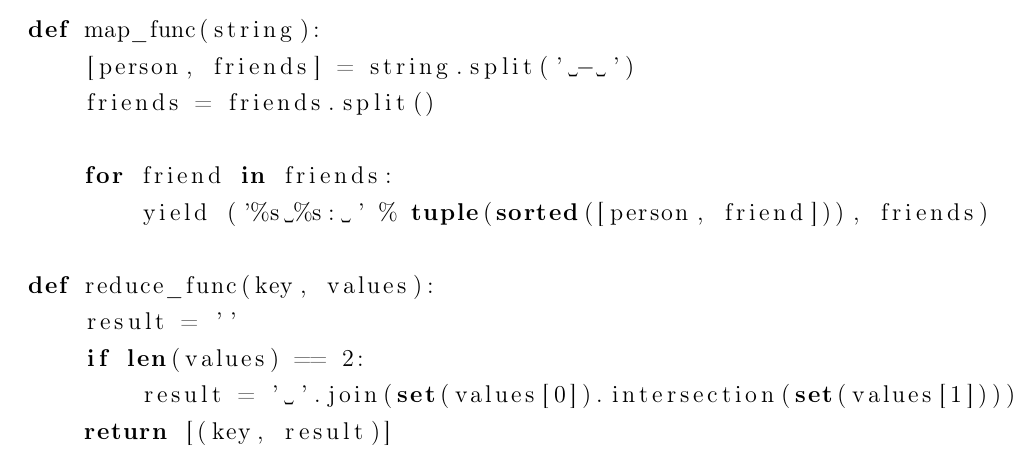
\includegraphics[scale=0.28]{code_sample.png}
        \end{figure}        
    \end{frame}
    
\section{Архитектура}

    \begin{frame}
    \frametitle{Архитектура распределённого map-reduce}
        \begin{figure}[h!]
            \centering
            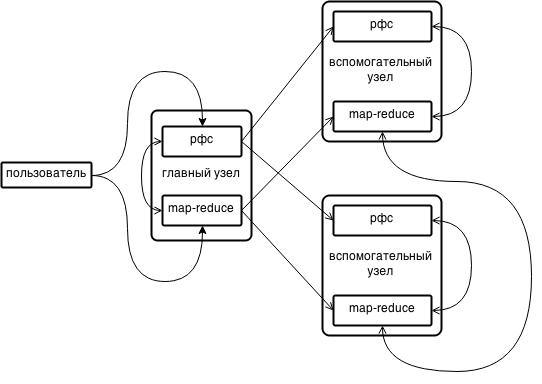
\includegraphics[scale=0.45]{framework_total.png}
        \end{figure}        
    \end{frame}

    \begin{frame}
    \frametitle{Архитектура распределённого map-reduce}
        \begin{figure}[h!]
            \centering
            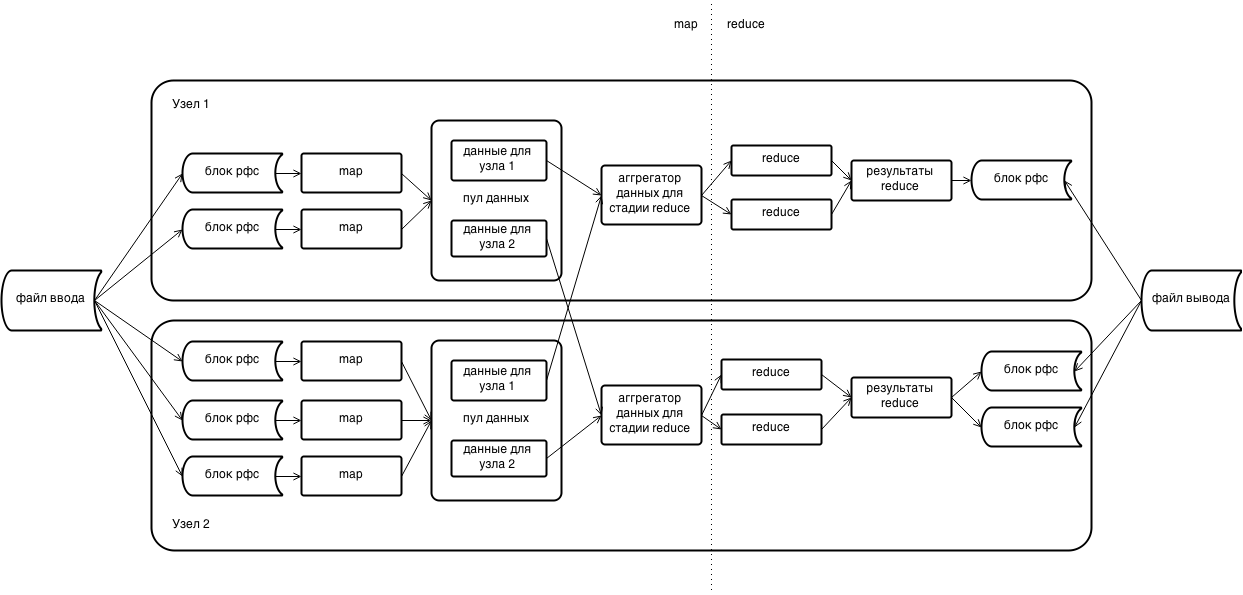
\includegraphics[scale=0.25]{map_reduce_framework.png}
        \end{figure}        
    \end{frame}

\section{Тестирование}
    \begin{frame}
    \frametitle{Результаты тестирования}
        \begin{figure}[h!]
            \centering
            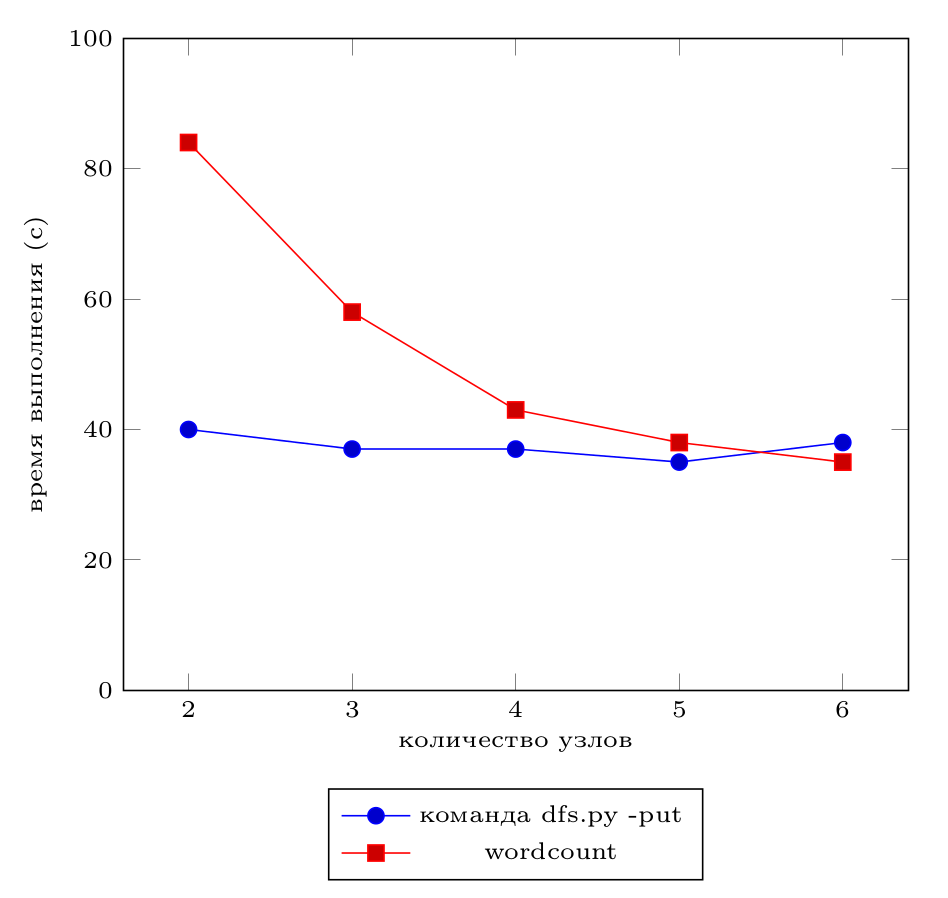
\includegraphics[scale=0.23]{test1.png}
        \end{figure}        
    \end{frame}

    \begin{frame}
    \frametitle{Результаты тестирования}
        \begin{figure}[h!]
            \centering
            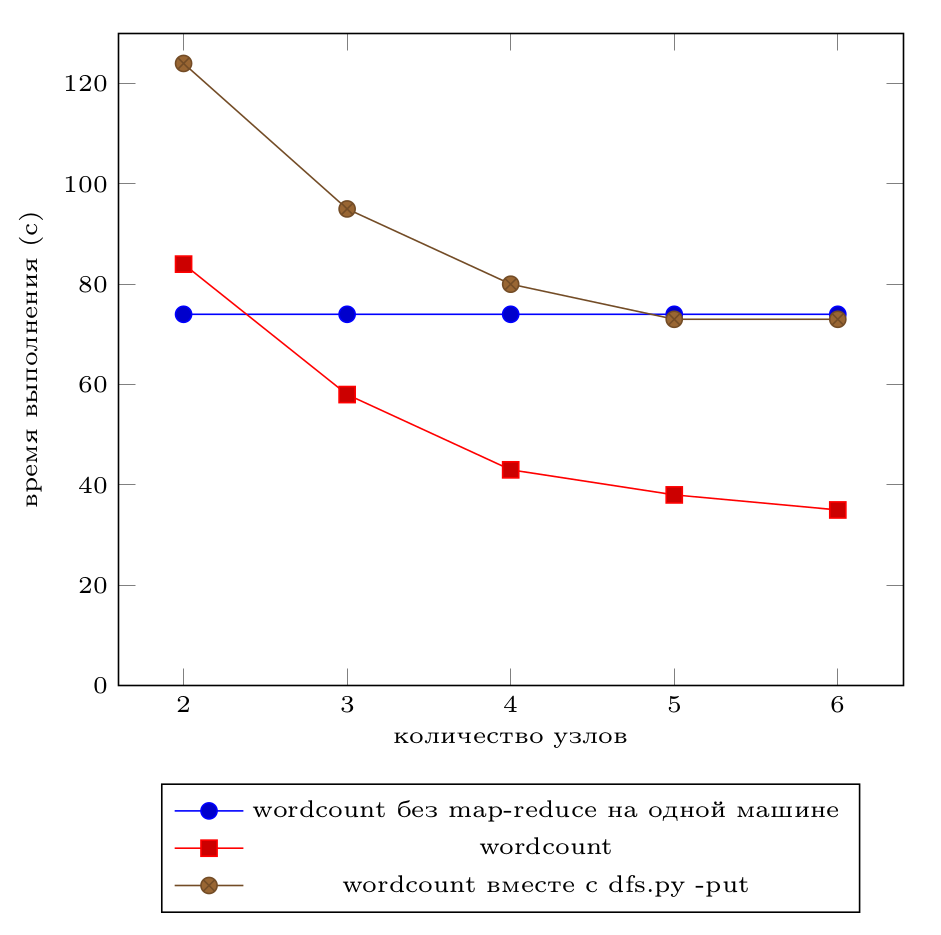
\includegraphics[scale=0.23]{test2.png}
        \end{figure}        
    \end{frame}

    \begin{frame}
    \frametitle{Результаты тестирования}
        \begin{itemize}
            \item Выполнение задачи класса информационный поиск:
            \begin{itemize}
                \item время загрузки данных в РФС~---~4мин.~30с.
                \item время выполнения задачи с помощью фреймворка map-reduce~---~1мин.~54с.
                \item время выполнения задачи на одной машине без использования фреймворка~---~6мин.~39с.
            \end{itemize}
        \end{itemize}
    \end{frame}

    \begin{frame}
    \frametitle{Выводы}
        \begin{itemize}
            \item С увеличением количества узлов производительность выполнения задач с помощью фреймворка растёт и превосходит производительность выполнения на одной машине.
            \item Время загрузки данных в РФС не зависит от количества узлов.
            \item Наиболее подходящей стратегий использования фреймворка является загрузка данных в РФС и их последующее использование в качестве входных данных для нескольких задач.
            \item Map-reduce удобная абстракция для построения решения части задач класса информационный поиск.
            \item Использование фреймфорка map-reduce для решения задач класса информационный поиск целесообразно.
        \end{itemize}
    \end{frame}

\begin{frame}
    \titlepage
\end{frame}

\end{document}